\documentclass{article}

\title{AI Jungle Docs}
\date{11-05-2024}
\author{EsharkyTheGreat}

\usepackage{amsmath}
\usepackage{listings}
\usepackage{minted}
\usepackage{tikz}
\usepackage{amsfonts}
\usepackage{pgfplots}

\pgfplotsset{compat=1.18}
\usetikzlibrary{decorations.pathreplacing}
\usetikzlibrary{positioning,calc}
\usetikzlibrary{backgrounds}
\usepgfplotslibrary{fillbetween}
\usetikzlibrary{patterns}
\pgfplotsset{compat=1.12}

\pgfmathdeclarefunction{gauss}{3}{%
  \pgfmathparse{1/(#3*sqrt(2*pi))*exp(-((#1-#2)^2)/(2*#3^2))}%
}
\pgfmathdeclarefunction{cdf}{3}{%
  \pgfmathparse{1/(1+exp(-0.07056*((#1-#2)/#3)^3 - 1.5976*(#1-#2)/#3))}%
}
\pgfmathdeclarefunction{fq}{3}{%
  \pgfmathparse{1/(sqrt(2*pi*#1))*exp(-(sqrt(#1)-#2/#3)^2/2)}%
}
\pgfmathdeclarefunction{fq0}{1}{%
  \pgfmathparse{1/(sqrt(2*pi*#1))*exp(-#1/2))}%
}

\def\N{50}
\colorlet{mydarkblue}{blue!30!black}



\begin{document}
\pagenumbering{gobble}
\maketitle
\newpage
\tableofcontents
\newpage
\pagenumbering{arabic}

\section{Probability}
\subsection{Introduction}
Probability is a measure of the likelihood that an event will occur. Probability is quantified as a number between 0 and 1, where 0 indicates impossibility and 1 indicates certainty. The higher the probability of an event, the more likely it is that the event will occur.

\paragraph{Frequentist Probability} fraction of times event occurs in experiment
\paragraph{Bayesian Probability} degree of belief in an event

\paragraph{Random Variable} X
\begin{description}
    \item[$\bullet$]Stochastic variable sampled from a set of possible
          outcomes
    \item [$\bullet$] Discrete or continuous E.g Labels like \{ Heads, Tails \} is discrete and gaussian distribution is continuous
    \item [$\bullet$] Probability distribution $ p(X) $
\end{description}

\subsection{Two Discrete Random Variables}
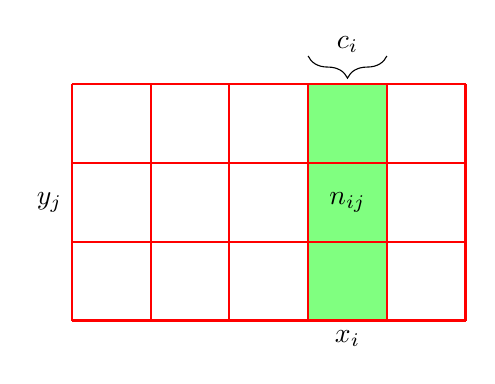
\begin{tikzpicture}
    % Draw the table

    % Highlight the cell n_ij
    \fill[green!50] (3,0) rectangle (4,3);
    % \fill[yellow!50] (3,2) rectangle (4,2);
    \draw[red, thick] (0,0) grid (5,3);

    % Label the cell n_ij
    \node at (3.5, 1.5) {$n_{ij}$};

    % Label y_j
    \node[anchor=east] at (0, 1.5) {$y_j$};

    % Label x_i
    \node[anchor=north] at (3.5, 0) {$x_i$};

    % Label the bracket for x_i column
    % \draw[thick] (3, 4.2) -- (4, 4.2);
    % \draw[thick] (3, 4.2) .. controls (3, 4.5) and (4, 4.5) .. (4, 4.2);
    % \node at (3.5, 3.5) {$c_i$};
    \draw [decorate,decoration={brace,amplitude=8pt,mirror,raise=4pt}] (3,3.5) -- (4,3.5) node[midway,yshift=0pt] {$c_i$};
    % Add vertical bracket for the rows
    % \draw[thick] (5.2, 0) -- (5.2, 4);
    % \draw[thick] (5.2, 0) .. controls (5.5, 0) and (5.5, 4) .. (5.2, 4);

\end{tikzpicture}
\begin{align*}
    x_i    & = \text{possible values of $X$}                  \\
    y_j    & = \text{possible values of $Y$}                  \\
    n_{ij} & = \text{number of times $X = x_i$ and $Y = y_j$} \\
    c_i    & = \text{number of times $X = x_i$}               \\
    N      & = \text{total number of samples}                 \\
\end{align*}

\paragraph{2 Random Variables X, Y}
\begin{center}
    $X = \{ x_1, x_2, x_3, x_4, x_5 \}$ \\
    $Y = \{ y_1, y_2, y_3 \}$
\end{center}

\paragraph{Joint Probability}
\begin{align*}
    p(X = x_i, Y = y_j) = n_{ij}/N
\end{align*}

\paragraph{Marginal Probability}
\begin{align*}
    p(X = x_i) & = c_i/N                                              \\
    c_i        & = \sum_{j=1}^{3} n_{ij}                              \\
    n_{ij}     & = p(X = x_i, Y = y_j)*N                              \\
    p(X = x_i) & = \frac{1}{N} \sum_{j=1}^{3} p(X = x_i, Y = y_j) * N \\
    p(X = x_i) & = \sum_{j=1}^{3} p(X = x_i, Y = y_j)
\end{align*}

\paragraph{Sum Rule}
\begin{align*}
    p(X = x_i) & = \sum_{Y} p(X = x_i, Y = y_j) \\
\end{align*}

\paragraph{Conditional Probability of Y given X}
\begin{align*}
    p(X = x_i)           & = \frac{c_i}{N}                                  \\
    p(Y = y_j | X = x_i) & = \frac{n_{ij}}{c_i}                             \\
    p(Y = y_j | X = x_i) & = \frac{p(X = x_i, Y = y_i) * N}{p(X = x_i) * N} \\
    p(Y = y_j | X = x_i) & = \frac{p(X = x_i, Y = y_j)}{p(X = x_i)}         \\
\end{align*}
\paragraph{Product Rule}
\begin{align*}
    p(X = x_i, Y = y_j) & = p(Y = y_j | X = x_i) * p(X = x_i) \\
    p(X = x_i, Y = y_j) & = p(X = x_i | Y = y_j) * p(Y = y_j) \\
\end{align*}

\subsection{Continuous Random Variables}
\begin{itemize}
    \item Probability of falling in the interval $(x, x+dx)$ is given
          by $p(x)dx$
    \item Here $p(x)dx$ is the probability density function over all possible x outputting the probability of its occurence
    \item Probability over finite interval $(a,b)$ is given by
          \begin{equation*}
              p(x \epsilon (a,b) ) = \int_{a}^{b}p(x)dx
          \end{equation*}
    \item Positivity
          \begin{equation*}
              p(x) \geq 0
          \end{equation*}
    \item Normalization
          \begin{equation*}
              \int_{-\infty}^{\infty}p(x)dx = 1
          \end{equation*}
    \item Change of variables - $x = g(y)$ probabilities in $(x,x+dx)$ must be transformed to $(y, y+dy)$
          \begin{align*}
              p_x(x)dx & = p_y(y)dy               \\
              p(y)     & = p(x) | \frac{dx}{dy} |
          \end{align*}
    \item Sum Rule
          \begin{equation*}
              p(x = x_i) = \int_{Y}^{} p(x=x_i,y)dy
          \end{equation*}
\end{itemize}

\subsection{Bayes Rule}
\begin{align*}
    p(y|x) & = \frac{p(x|y)p(y)}{p(x)} \\
\end{align*}
\begin{itemize}
    \item $p(y|x)$ - is the posterior probability of Y=y
    \item $p(x|y)$ - is the likelihood of X=x given Y=y
    \item $p(y)$ - is the prior probability of Y=y
    \item $p(x)$ - is the evidence for X=x
\end{itemize}

\subsection{Expectation}
Random Variable $x$ $\epsilon$ $X$ and function $ f : X \rightarrow R $
\begin{align*}
    \mathbb{E}[f]           & = \mathbb{E}_{x \sim p(X)}[f(x)]          \\
    \mathbb{E}[f(x)]        & = \sum_{x} f(x)p(x) \quad \text{Discrete} \\
    \mathbb{E}[f(x)]        & = \int f(x)p(x)dx \quad \text{Continuous} \\
    \mathbb{E}[f(x) + g(x)] & = \mathbb{E}[f(x)] + \mathbb{E}[g(x)]     \\
    \mathbb{E}[cf(x)]       & = c\mathbb{E}[f(x)]                       \\
\end{align*}

\subsection{Variance}
The variance of a random variable is a measure of how much the values of the variable vary as we sample different values of the variable from its probability distribution. \\
The expected quadratic distance of the random variable from its mean.
\begin{align*}
    Var[f]           & = \mathbb{E}[(f(x) - \mathbb{E}[f(x)])^2]                                     \\
    Var[f]           & = \mathbb{E}[f(x)^2 - 2f(x)\mathbb{E}[f(x)] + \mathbb{E}[f(x)]^2 ]            \\
    \mathbb{E}[f(x)] & = constant                                                                    \\
    Var[f]           & = \mathbb{E}[f(x)^2] - 2\mathbb{E}[f(x)]\mathbb{E}[f(x)] + \mathbb{E}[f(x)]^2 \\
    Var[f]           & = \mathbb{E}[f(x)^2] - \mathbb{E}[f(x)]^2                                     \\
\end{align*}

\subsection{Covariance}
Measure of how much two random variables change together
\begin{align}
    Cov[x,y] & = \mathbb{E}[(x - \mathbb{E}[x])(y - \mathbb{E}[y])]                          \\
    Cov[x,y] & = \mathbb{E}[xy -x\mathbb{E}[y] -y\mathbb{E}[x] + \mathbb{E}[x]\mathbb{E}[y]] \\
    Cov[x,y] & = \mathbb{E}[xy] - \mathbb{E}[x]\mathbb{E}[y]                                 \\
\end{align}
Independent Random Variables $p(x,y)=p(x)p(y)$ \\
Covariance doesn't imply that variables are independant

\subsection{Gaussian Distribution}
\begin{center}
    \begin{tikzpicture}
        \message{68-95-99 rule^^J}

        \def\B{11};
        \def\Bs{3.0};
        \def\xmax{\B+3.2*\Bs};
        \def\ymin{{-0.1*gauss(\B,\B,\Bs)}};
        \def\h{0.08*gauss(\B,\B,\Bs)};

        \begin{axis}[every axis plot post/.append style={
            mark=none,domain={-0.05*(\xmax)}:{1.08*\xmax},samples=\N,smooth},
            xmin={-0.1*(\xmax)}, xmax=\xmax,
            ymin=\ymin, ymax={1.1*gauss(\B,\B,\Bs)},
            axis lines=middle,
            axis line style=thick,
            enlargelimits=upper, % extend the axes a bit to the right and top
            ticks=none,
            xlabel=$x$,
            every axis x label/.style={at={(current axis.right of origin)},anchor=north},
            width=0.85*\textwidth, height=0.55*\textwidth,
            y=700pt,
            clip=false
            ]

            % PLOTS
            \addplot[blue,thick,name path=B] {gauss(x,\B,\Bs)};

            % FILL
            \path[name path=xaxis]
            (0,0) -- (\pgfkeysvalueof{/pgfplots/xmax},0); %\pgfkeysvalueof{/pgfplots/xmin}
            \addplot[blue!50] fill between[of=xaxis and B, soft clip={domain={\B-3*\Bs}:{\B+3*\Bs}}];
            \addplot[blue!25] fill between[of=xaxis and B, soft clip={domain={\B-2*\Bs}:{\B+2*\Bs}}];
            \addplot[blue!10] fill between[of=xaxis and B, soft clip={domain={\B-1*\Bs}:{\B+1*\Bs}}];

            % LINES
            \addplot[black,dashed,thick]
            coordinates {({\B-3*\Bs},{20*gauss(\B-3*\Bs,\B,\Bs)}) ({\B-3*\Bs},{-\h})}
            node[below=-3pt,scale=0.8] {\strut$\mu-3\sigma$};
            \addplot[black,dashed,thick]
            coordinates {({\B-2*\Bs},{4*gauss(\B-2*\Bs,\B,\Bs)}) ({\B-2*\Bs},{-\h})}
            node[below=-3pt,scale=0.8] {\strut$\mu-2\sigma$};
            \addplot[black,dashed,thick]
            coordinates {({\B-1*\Bs},{1.3*gauss(\B-\Bs,\B,\Bs)}) ({\B-1*\Bs},{-\h})}
            node[below=-3pt,scale=0.8] at ({\B-\Bs},{-\h}) {\strut$\mu-\sigma$};
            \addplot[black,dashed,line width=0.7pt]
            coordinates {(\B,{1.05*gauss(\B,\B,\Bs)}) (\B,{-\h})}
            node[below=-3pt,scale=0.8] {\strut$\mu$};
            \addplot[black,dashed,thick]
            coordinates {({\B+1*\Bs},{1.3*gauss(\B+\Bs,\B,\Bs)}) ({\B+1*\Bs},{-\h})}
            node[below=-3pt,scale=0.8] at ({\B+\Bs},{-\h}) {\strut$\mu+\sigma$};
            \addplot[black,dashed,thick]
            coordinates {({\B+2*\Bs},{4*gauss(\B+2*\Bs,\B,\Bs)}) ({\B+2*\Bs},{-\h})}
            node[below=-3pt,scale=0.8] at ({\B+2*\Bs},{-\h}) {\strut$\mu+2\sigma$};
            \addplot[black,dashed,thick]
            coordinates {({\B+3*\Bs},{20*gauss(\B+3*\Bs,\B,\Bs)}) ({\B+3*\Bs},{-\h})}
            node[below=-3pt,scale=0.8] at ({\B+3*\Bs},{-\h}) {\strut$\mu+3\sigma$};

            % AREAS
            \addplot[<->,mydarkblue,thick]
            coordinates {({\B-\Bs},{.55*gauss(\B,\B,\Bs)}) ({\B+\Bs},{.55*gauss(\B,\B,\Bs)})};
            \addplot[<->,mydarkblue,thick]
            coordinates {({\B-2*\Bs},{.35*gauss(\B,\B,\Bs)}) ({\B+2*\Bs},{.35*gauss(\B,\B,\Bs)})};
            \addplot[<->,mydarkblue,thick]
            coordinates {({\B-3*\Bs},{.15*gauss(\B,\B,\Bs)}) ({\B+3*\Bs},{.15*gauss(\B,\B,\Bs)})};
            \node[mydarkblue,fill=blue!10,inner xsep=3,inner ysep=1,scale=1]
            at (\B,{.55*gauss(\B,\B,\Bs)}) {68.3\%};
            \node[mydarkblue,fill=blue!10,inner xsep=3,inner ysep=2,scale=1]
            at (\B,{.35*gauss(\B,\B,\Bs)}) {95.5\%};
            \node[mydarkblue,fill=blue!10,inner xsep=3,inner ysep=2,scale=1]
            at (\B,{.15*gauss(\B,\B,\Bs)}) {99.7\%};

        \end{axis}
    \end{tikzpicture}

\end{center}
\begin{align*}
    p(x)                        & = \frac{1}{\sqrt{2\pi\sigma^2}}exp{-\frac{(x-\mu)^2}{2\sigma^2}} \\
    \mathcal{N}(x|\mu,\sigma^2) & = \text{Normal Distribution}                                     \\
    \mu                         & = \text{mean}                                                    \\
    \sigma^2                    & = \text{variance}                                                \\
\end{align*}
Since this is a probability distribution it should be normalized that is with respect to the function $f(x) = 1$ the expected value should be 1 or the area under the curve of this distribution should be one
\begin{align*}
    \int_{-\infty}^{\infty} \frac{1}{\sqrt{2\pi\sigma^2}}exp(-\frac{(x-\mu)^2}{2\sigma^2})dx & = 1
\end{align*}
\subsubsection{Mean}
\begin{align*}
    \mathbb{E}[x] & = \int_{-\infty}^{\infty} x\mathcal{N}(x|\mu,\sigma^2)dx \\
    \mathbb{E}[x] & = \mu
\end{align*}
\subsubsection{Variance}
\begin{align*}
    Var[x] & = \mathbb{E}[(x-\mathbb{E}[x])^2]                                \\
    Var[x] & = \int_{-\infty}^{\infty} (x-\mu)^2\mathcal{N}(x|\mu,\sigma^2)dx \\
    Var[x] & = \sigma^2
\end{align*}
\subsubsection{Multivariate Gaussian Distribution}

$x$ is a $D$-dimensional vector $x = (x_1, x_2, x_3, ..., x_D)^ T$
\begin{align*}
    p(x)          & = \frac{1}{(2\pi)^{D/2}|\Sigma|^{1/2}}exp(-\frac{1}{2}(x-\mu)^T\Sigma^{-1}(x-\mu)) \\
    \Sigma        & = \text{Covariance Matrix}                                                         \\
    \Sigma        & = cov[x,x]                                                                         \\
    \mathbb{E}[x] & = \int x\mathcal{N}(x|\mu,\Sigma)dx                                                \\
                  & = \mu
\end{align*}

\subsection{Maximum Likelihood Principle}
\begin{itemize}
    \item Given a dataset $D = (x_1, x_2, x_3, ..., x_N)$ and a model $p(x|\theta)$ the likelihood of the model is given by $p(D|\theta)$ where $\theta$ is the parameter of the model
    \item The maximum likelihood estimate of $\theta_{ml}$ is the value that maximizes the likelihood of the model given the data
          \begin{equation*} \theta_{ml} = \operatorname*{arg\,max}_\theta  p(D|\theta) \end{equation*}
    \item We assume $(x_1, x_2 , ... , x_N$) are independent and identically distributed
          \begin{align*}
              p(D|\theta) =                                 & \prod_{n=1}^{N}p(x_n|\theta) \\
              \theta_{ml} = \operatorname*{arg\,max}_\theta & \prod_{n=1}^{N}p(x_n|\theta) \\
          \end{align*}
    \item Instead of likelihood we maximize log likelihood as probabilities multiplied together will result in a very small number, it can be proven that taking log doesnt affect the result
          \begin{align*}
              \theta_{ml} = \operatorname*{arg\,max}_\theta & (log(\prod_{n=1}^{N}p(x_n|\theta))) \\
              \theta_{ml} = \operatorname*{arg\,max}_\theta & \sum_{n=1}^{N}log(p(x_n|\theta))    \\
          \end{align*}
\end{itemize}
\subsubsection{Maximum Likelihood for Gaussian Distribution}
\begin{align*}
    p(x|\mu,\sigma^2)      & = \frac{1}{\sqrt{2\pi\sigma^2}}exp(-\frac{(x-\mu)^2}{2\sigma^2}) \\
    p(D|\mu,\sigma^2)      & = \prod_{n=1}^{N}p(x_n|\mu,\sigma^2)                             \\
    log(p(D|\mu,\sigma^2)) & = \sum_{n=1}^{N}log(p(x_n|\mu,\sigma^2))                         \\
\end{align*}
For finding the maximum likelihood estimate we take the derivative of the log likelihood with respect to the parameters and set them to zero
\begin{align*}
    \frac{\partial}{\partial \mu}log(p(D|\mu,\sigma^2))      & = 0 \\
    \frac{\partial}{\partial \sigma^2}log(p(D|\mu,\sigma^2)) & = 0 \\
\end{align*}
Solving this we get the maximum likelihood estimate of the parameters
\begin{align*}
    \mu_{ml}      & = \frac{1}{N}\sum_{n=1}^{N}x_n              \\
    \sigma^2_{ml} & = \frac{1}{N}\sum_{n=1}^{N}(x_n-\mu_{ml})^2
\end{align*}

\newpage
\section{Statistics}
\subsection{Correlation}
\paragraph{Pearson's Correlation Coefficient} The correlation coefficient ranges from –1 to 1. When it is close to 1, it means that
there is a strong positive correlation; for example, the median house value tends to go
up when the median income goes up. When the coefficient is close to –1, it means
that there is a strong negative correlation; you can see a small negative correlation
between the latitude and the median house value (i.e., prices have a slight tendency to
go down when you go north). Finally, coefficients close to zero mean that there is no
linear correlation

\newpage
\section{Data Processing}
\subsection{Data Splitting}
It is important that we immediately split the data into training and testing sets so that there is no
data snooping bias (Our brain always looks at pattern and is good at overfitting therefore when we look at the whole data we might apply techniques that overfit the data and the model becomes unusable).

\subsubsection{Random Splitting}
We take a random seed and split the data into training and testing sets. But the problem is that
the data might not be evenly distributed and if we add more data the split might change due to this
some data in the original training set will come in the testing set causing bias.
\begin{minted}[frame=lines]
{python3}
import numpy as np

def split_train_test(data, test_ratio):
    np.random.seed(42)
    shuffled_indices = np.random.permutation(len(data))
    test_set_size = int(len(data) * test_ratio)
    test_indices = shuffled_indices[:test_set_size]
    train_indices = shuffled_indices[test_set_size:]
    return data.iloc[train_indices], data.iloc[test_indices]
\end{minted}
\subsubsection{Checksum Splitting}
We calculate the hash of the data and split the data based on the hash. This way the data will always be split the same way and we can add new data without worrying
about the split changing.
\begin{minted}[frame=lines]
{python3}
from zlib import crc32

    def test_set_check(identifier, test_ratio):
        return crc32(np.int64(identifier)) & 0xffffffff < test_ratio * 2**32
    def split_train_test_by_id(data, test_ratio, id_column):
        ids = data[id_column]
        in_test_set = ids.apply(lambda id_: test_set_check(id_, test_ratio))
        return data.loc[~in_test_set], data.loc[in_test_set]
\end{minted}
\subsubsection{Stratified Splitting}
\begin{minipage}{\textwidth}
    When we want the same distribution of categorical data in the main dataset to be present in both the training and testing data set because of the importance of the distribution to the model we use Stratified Splitting
    \begin{minted}[frame=lines]
{python3}
from sklearn.model_selection import StratifiedShuffleSplit

split = StratifiedShuffleSplit(n_splits=1, test_size=0.2, random_state=42)
for train_index, test_index in split.split(housing, housing["income_cat"]):
    strat_train_set = housing.loc[train_index]
    strat_test_set = housing.loc[test_index]
\end{minted}
\end{minipage}
\newpage

\newpage

\section{Machine Learning}

\subsection{Linear Regression}
\subsection{Logistic Regression}
\subsection{Error}

\paragraph{Root Mean Square Error (RMSE) - L2 Norm}
\begin{equation}
    RMSE = \sqrt{\frac{1}{n}\sum_{i=1}^{n}(h(x_i) - \hat{y_i})^2}
\end{equation}
\begin{align*}
    where, \quad h(x_i) & = \text{predicted value}     \\
    h                   & = \text{hypothesis function} \\
    \hat{y_i}           & = \text{actual value}        \\
\end{align*}
This is useful when you want to know how far off your predictions are from the actual values.
Cases where the model is far from the correct value is treated more harshly then the cases that are nearby but not exactly correct.


\paragraph{Mean Absolute Error (MAE) - L1 Norm}
\begin{equation}
    MAE = \frac{1}{n}\sum_{i=1}^{n}|h(x_i) - \hat{y_i}|
\end{equation}
\begin{align*}
    where, \quad h(x_i) & = \text{predicted value}     \\
    h                   & = \text{hypothesis function} \\
    \hat{y_i}           & = \text{actual value}        \\
\end{align*}
We mostly use RMSE but when there are too many outlier cases that we can't have the model be harsh on all of them we use MAE that averages out the error.

\newpage
\section{Python Tips and Tricks}
\subsection{Sklearn}
\subsection{Matplot}
\subsection{Numpy}
\subsection{Pandas}


\end{document}